% Created 2021-09-28 Tue 18:31
% Intended LaTeX compiler: pdflatex
\documentclass[11pt]{article}
\usepackage[utf8]{inputenc}
\usepackage[T1]{fontenc}
\usepackage{graphicx}
\usepackage{grffile}
\usepackage{longtable}
\usepackage{wrapfig}
\usepackage{rotating}
\usepackage[normalem]{ulem}
\usepackage{amsmath}
\usepackage{textcomp}
\usepackage{amssymb}
\usepackage{capt-of}
\usepackage{hyperref}
\usepackage{minted}
\usepackage[utf8]{inputenc}
\usepackage[dvipsnames]{xcolor}
\usepackage{tikz}
\usepackage{pdfpages}
\usepackage[, germanb]{babel}
\usepackage{listings}
\usepackage[]{babel}
\usepackage[dvipsnames]{xcolor}
\usepackage{courier}
\usepackage{listings}
\usepackage{textcomp}
\usepackage{gensymb}
\author{Jakob Klemm, Dominik Keller}
\date{}
\title{Projekt Orion}
\hypersetup{
 pdfauthor={Jakob Klemm, Dominik Keller},
 pdftitle={Projekt Orion},
 pdfkeywords={},
 pdfsubject={},
 pdfcreator={Emacs 28.0.50 (Org mode 9.4.4)}, 
 pdflang={Germanb}}
\begin{document}

\maketitle
\tableofcontents

\newpage  
\begin{ABSTRACT}
TODO: Abstract
\end{ABSTRACT}
\newpage

\textbf{Vorwort}\\
Die schriftliche Komponente der Maturaarbeit \texttt{Projekt Orion} besteht aus
drei verschiedenen Teilen. Da die behandelten Themen äusserst komplex
und umfangreich sind, verlangen verschiedene Abschnitte der Arbeit
verschiedenes Vorwissen und einen verschiedenen Zeitaufwand. Deswegen
wurde die schriftliche Komponente in drei Subkomponenten aufgeteilt,
wobei sie nach technischem Detailgrad sortiert sind. Wer nur ein
oberflächliches Verständnis über die Arbeiten und eine Analyse des
Umfelds will, ohne dabei zu technisch zu werden, muss nicht über den
Umfang dieses Dokuments hinaus. Aber für vollständigen Einblick in die
Errungenschaften und Konzepte muss mit einem grösseren Aufwand
gerechnet werden.
\begin{itemize}
\item Schriftlicher Kommentar: In diesem Dokument hier findet sich eine
klassische Besprechung der Arbeit. Begonnen mit einer Zielsetzung
und Besprechung verschiedener Projekte, bis zur Analyse des Produkts
und einem Ausblick in die Zukunft gibt dieses Dokument einen guten,
aber oberflächlichen Einblick in das \texttt{Projekt Orion}. Natürlich wird
besonders bei der Analyse der existierenden Projekten und Darlegung
des Konzepts gewisses technisches Know-How benötigt, aber es wurde
versucht, alle Fachbegriffe zu umschreiben oder zu erklären. Wer nur
über die Vision und den aktuellen Stand wissen will muss nicht über
dieses Dokument hinaus, aber verschiedene Konzepte und nahezu die
gesamte technische Umsetzung befinden sind nicht in diesem Dokument.
\item Dokumentation: In dieser alleinstehenden Dokumentation, welche im
Detailgrad zwischen dem schriftlichen Kommentar und der
Code-Dokumentation steht, werden die Konzepte und Ideen besprochen.
Wer die Entstehung und aktuelle Form der Komponenten genauer
verstehen will, oder wer von den umgesetzten Funktionen profitieren
will, sollte die Dokumentation durcharbeiten. Das Dokument ist eher
umfangreich, es kann aber auch gut als eine Art Nachschlagewerk
verwendet werden.
\item Code: Neben der Dokumentation des Projekts und der Konzepte,
existiert eine weitere Form der Dokumentation. Nahezu jede Funktion,
jedes Modul und jedes Objekt über die verschiedenen \emph{Crates} sind
dokumentiert. Diese Dokumentationen lassen sich nicht in einem
klassisch strukturierten Dokument finden. Stattdessen ist die
Code-Dokumentation online über automatisch generierte
Rust-Dokumentation zu finden. Die Seiten mögen anfangs etwas
unübersichtlich wirken, wer aber den Code von \texttt{Projekt Orion}
verwenden will wird sich dort gut zurecht finden.
\end{itemize}
\newpage

\section{Vision}
\label{sec:org7738f31}
\subsection{Grenzen}
\label{sec:org1d76eb9}
\subsection{Inhalte}
\label{sec:org23ba6ea}
\subsection{Routing}
\label{sec:orga86dedb}
\subsection{Zentralisierung}
\label{sec:org1f02809}
\subsection{Orion}
\label{sec:orgc8ad0fe}
\section{Projekte}
\label{sec:orgf338f0a}
\subsection{Kademlia}
\label{sec:orgfe83447}
Wie geht man also gegen die totale Abhängikeit von Internetanbietern
und zentralen Routern vor?\\
Man kann ja nicht einfach seine eigenen Router aufsetzen und einen
alternativen Dienst anbieten. Neben den technischen Schwierigkeiten
würde ein solcher Schritt auch überhaupt nichts das eigentliche
Problem bekämpfen.\\

\noindent Der Trick, der bei Systemen wie \texttt{Kademlia} verwendet wird, ist
es, Router vollständig zu eliminieren. Dies ist möglich, indem jedes
Mitglied des Netzwerks neben seinen normalen Funktionen gleichzeitig
auch noch als Router agiert. Strenggenommen werden in \texttt{Kademlia} Router
also nicht wirklich eliminiert, lediglich zentrale Router fallen
weg.\\

\noindent In einem früheren Abschnitt wurden die Probleme der
\emph{Zentralrouter} bereits angesprochen. Wenn jetzt aber jedes Mitglied in
einem Netzwerk plötzlich als Router agiert und es keine zentrale
Instanz gibt, träfe die Problematik der \emph{Zentralrouter} plötzlich auf
alle Server zu. Genau da kommt \texttt{Kademlia} ins Spiel. Aber was genau ist
\texttt{Kademlia} eigentlich?\\

\noindent Laut den Erfindern, \emph{Petar Maymounkov} und \emph{David Mazières},
ist es
\begin{center}
ein Peer-to-peer Nachrichten System basierend auf XOR-Metrik.\footnote{Kademlia: Whitepaper:
\url{https://pdos.csail.mit.edu/\~petar/papers/maymounkov-kademlia-lncs.pdf},
heruntergeladen am: 30.05.2020.}
\end{center}
Was genau bedeutet das und wie lässt sich eine \texttt{XOR}-Metrik für
verteilte Datensysteme einsetzen?\\

\noindent Da die einzelnen Server nicht in der Lage sind,
Informationen über das komplette Netzwerk zu speichern oder zu
verarbeiten, funktionieren \texttt{Kademlia}-Systeme grundlegend anders.
Anstelle der hierarchischen Anordnung der Router ist jedes Mitglied
eines Systems gleichgestellt. dabei kümmert sich jedes Mitglied auch
nicht um das komplette System, sondern nur um sein direktes Umfeld.
Während dies für kleinere Systeme gut funktioniert und vergleichbare
Geschwindigkeiten liefert, skaliert es nicht so einfach für grosse
Systeme. Genau dafür gibt es die \texttt{XOR}-Metrik.
\subsubsection{Distanz}
\label{sec:org7440489}
Die \texttt{XOR}-Funktion, die in der Informatik an den verschiedensten
Orten auftaucht, wird verwendet, um die Distanz zwischen zwei
Zahlen zu berechnen. Die Zahlen repräsentieren dabei Mitglieder
im Netzwerk und sind je nach Variante im Bereich
\(0..2^{160}\)(\emph{20 Bytes}) oder \(0..2^{256}\)(\emph{32 Bytes}). Mit einem
so grossen Bereich lässt sich auch das Problem der limitierten
\texttt{IP-Adressen} lösen. Auch wenn es kein tatsächlich unlimitiertes
System ist, so gibt es doch mehr als genug Adressen.\\

\noindent Wenn mit \texttt{XOR}-Funktionen einfach die Distanz zwischen
zwei Zahlen berechnet wird, stellt sich die Frage, wieso nicht
einfach die Differenz verwendet wird. Um dies zu beantworten,
muss man sich die Eigenschaften der \texttt{XOR}-Funktion etwas genauer
anschauen:

\begin{enumerate}
\item \(xor(x, x) = 0\): Das Mitglied mit seiner eigenen Adresse ist
zu sich selbst am nächsten. Mitglieder werden hier als Namen
für Server in einem \texttt{Kademlia}-System verwendet.
\item \(xor(x, y) > 0\) wenn \(x \neq y\): Die Funktion produziert nie
negative Zahlen und nur mit zwei identischen Parametern kann
man \(0\) erhalten.
\item \(xor(x, y) = xor(y, x)\): Die Reihenfolge der Parameter spielt
keine Rolle.
\item \(xor(x, z) \leq xor(x, y) + xor(y, z)\): Die direkte Distanz
zwischen zwei Punkten ist am kürzesten oder gleich kurz wie
die Distanz mit einem zusätzlichen Schritt dazwischen, also
einem weiteren Sprung im Netzwerk.
\item Für ein gegebenes \(x\) und eine Distanz \(l\) gibt es nur
genau ein \(y\) für das \(xor(x, y) = l\) gilt.
\end{enumerate}

\noindent Aber wieso genau funktioniert dies? Wieso kann man \texttt{XOR}, eine
Funktion zur Berechnung der Bit-Unterschiede in zwei Binärzahlen,
verwenden, um die Distanz zwischen zwei Punkten in einem verteilten
Datensystem zu berechnen?\\

\noindent Um dies zu verstehen, hilft es, sich das System als
umgekehrten Baum vorzustellen. Untergeordnet zum zentralen Punkt zu
oberst stehen alle Mitglieder im System. Mit jeder weiteren Abzweigung
zweier Teilbäume halbiert sich die Anzahl. Man wählt am einfachsten
zwei Abzweigungen pro Knoten, da sich damit die Werte direkt als
Binärzahlen darstellen lassen, wobei jeder Knotenpunkt einfach eine
Stelle in der langen Kette aus \(0\) oder \(1\) darstellt. Der ganze
Baum sieht dann wie folgt aus\footnote{Wikipedia: Kademlia \url{https://en.wikipedia.org/wiki/Kademlia},
heruntergeladen am: 30.05.2020.}:

\begin{center}
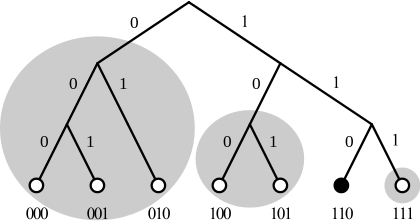
\includegraphics[width=.9\linewidth]{tree.png}
\captionof{figure}{Beispielhafte Darstellung eines einfachen Kademlia-Systems}
\end{center}

\noindent Mit dieser Sicht auf das System beschreibt die \texttt{XOR}-Funktion
die Anzahl der unterschiedlichen Abbiegungen im Baum und somit die
Distanz. Zwar mag es auf den ersten Blick nicht intuitiv wirken, wieso
man \texttt{XOR} anstatt einfach der Differenz verwendet, allerdings
funktioniert die Funktion mit Binärzahlen in einem solchen Baum
einiges besser.
\subsubsection{Routing-Table}
\label{sec:orgb6ad648}
In einem \texttt{Kademlia}-System hat jedes Mitglied eine gewisse Anzahl
anderer Mitglieder, mit denen es sich verbunden hat. Da \texttt{Kademlia} ein
sehr umfangreiches, kompliziertes Protokoll und System beschreibt,
sollen hier nur einige zentrale Funktionen besprochen werden, die für
diesen ersten Prototypen von \texttt{Engine: Orion} relevant sind. Besonders
beim \texttt{Routing Table} lassen sich einige Abschnitte weglassen, welche
zwar für die Optimierung und Skalierung eines Systems wichtig,
allerdings für das Analysieren eines einfachen, kleinen Systems wie
\texttt{Engine: Orion} irrelevant sind.\\

\noindent Einfach formuliert speichert der \texttt{Routing Table} die
verbundenen Mitglieder. Eine eingehende Nachricht wird dann mithilfe
dieser Liste, sowie der \texttt{XOR}-Metrik ans richtige Ziel geschickt. Um das
System zu optimieren und die Anzahl der benötigten Sprünge klein zu
halten, wird ein spezielles System verwendet, um zu entscheiden,
welche Mitglieder im \texttt{Routing-Table} gespeichert werden sollen:

\begin{enumerate}
\item Sehr nahe an sich selbst (in der obigen Darstellung also:
wenige Sprünge im Baum) werden alle Mitglieder gespeichert.
\item Je weiter weg sich die Mitglieder befinden, desto weniger
werden gespeichert.
\end{enumerate}

\noindent Die optimale Anzahl der gespeicherten Mitglieder hängt von
den Zielen und Ansprüchen an das System ab. Grundlegend muss man die
Frage beantworten, mit wie vielen Unterbäumen Verbindungen gehalten
werden sollen. Zwar mag dies etwas abstrakt wirken, es lässt sich aber
mit dem eben eingeführten Modell eines umgekehrten Baumes gut
erklären:
\begin{itemize}
\item In der obersten Ebene trennt sich der Baum in zwei vollständig
getrennte Teile, was sich mit jeder weiteren Ebene wiederholt.
\item Die einzige Möglichkeit vom einen \emph{Ende} des Baums zum anderen
zu kommen, ist über den obersten Knoten. Um also in die andere
Hälfte zu kommen, braucht man mindestens eine Verbindungsstelle
in der anderen Hälfte.
\item Deshalb braucht ein \texttt{Routing-Table} nicht nur kurze
Verbindungen zu nahen Punkten, sondern auch einige wenige
Verbindungen zu Mitgliedern in der anderen Hälfte.
\item Mit nur einer weit entfernten Adresse hat man eine Verbindung
in \emph{eigene} und die \emph{andere} Hälfte. Hat man zwei solche
Verbindungen auf die andere Seite hat man schon Verbindungen in
jeden Viertel des Baumes.
\item Man muss also entscheiden, wie fein man die andere Hälfte
aufteilen will. (Eine genaue Unterteilung bedeutet wenige
Sprünge aber grosse \texttt{Routing-Tables}, eine grobe Unterteilung
genau das Umgekehrte).
\end{itemize}

\noindent Zwar hat ein vollständiges \texttt{Kademlia}-System noch
komplexere Elemente, wie \texttt{k-Buckets}, welche den \texttt{Routing-Table}
optimieren, allerdings sind diese für die grundlegende
Funktionsweise des Systems irrelevant.\\

\noindent Die dynamische Regulation des \texttt{Routing-Tables} muss
allerdings noch erwähnt werden:
\begin{itemize}
\item Sobald die definierte Maximalgrösse erreicht ist, werden keine
neuen Verbindungen akzeptiert.
\item Zwar können existierende Einträge durch Neue ersetzt werden,
allerdings werden dabei nicht alte, sondern inaktive Einträge
entfernt. Für ein \texttt{Kademlia}-System werden also auch Mechanismen
benötigt, um die Zustände aller Verbindungen periodisch zu
überprüfen.
\end{itemize}
\subsection{BitTorrent}
\label{sec:org73f4d39}
Dezentralisierung hat viele Vorteile und muss langfristig
flächendeckend eingesetzt werden. Aktuell sind die meisten
Industrien und Produkte noch nicht so weit. Trotzdem gibt es
einige Anwendungen und Gruppen bei denen solche Systeme bereits
seit Jahren Verwendung finden.\\

\noindent Beispielsweise im Zusammenhang mit \emph{(mehr oder weniger
legalen)} Verbreiten von Materialien wie Filmen oder Musik wird
eines der grössten global verteilten Systeme eingesetzt. Natürlich
gibt es hunderte von verschiedenen Programmen, Ideen und
Umsetzungen, wobei die meisten Nachfolger von \texttt{Napster} sind.\\

\noindent Im preisgekrönten Film \emph{The social network} erhält man
Einblick in den Lebensstil von \texttt{Sean Parker}, einem der Gründer von
\texttt{Napster}. Es mag überraschen, wie jemand wie Parker, der nur wenige
Jahre zuvor mit \texttt{Napster} die komplette Musikindustrie in Unruhe
gebracht hatte, eine so zentrale Rolle in \texttt{Facebook}, einem der
zentralisiertesten Megaunternehmen der Welt, einnehmen konnte.\\

\noindent Auch wenn es noch nicht \emph{vollständig} dezentralisiert ist,
erlaubte es \texttt{Napster} Nutzern, Musik über ein automatisiertes System
mit anderen Nutzern zu teilen und neue Titel direkt von den
Geräten anderer Nutzer herunterzuladen. Dabei gab es allerdings
immer noch einen zentralen Server, der die Titel sortierte und
indizierte. \\
\texttt{Napster} musste am Ende abgeschaltet werden, nachdem die Klagen der
Musikindustrie zu belastend wurden. Auch wenn das Produkt
abgeschaltet wurde, liess sich nichts mehr gegen die Idee
unternehmen.\\

\noindent Über viele Iterationen und Generationen hinweg wurden
die verteilten Systeme immer weiter verbessert, jegliche zentrale
Server entfernt und in die Hände immer mehr Nutzer gebracht. Heute
läuft ein Grossteil des Austauschs über \texttt{BitTorrent}.

\noindent \texttt{BitTorrent} baut auf der gleichen grundlegenden Idee wie
\texttt{Napster} auf: Nutzer stellen ihren eigenen Katalog an Medien zur
Verfügung und können Inhalte von allen anderen Mitgliedern im
System herunterladen. Anders als \texttt{Napster} gibt es bei \texttt{BitTorrent}
keine zentrale Komponente, stattdessen findet selbst das
Indizieren und Finden von Inhalten dezentralisiert statt\footnote{BitTorrent: Mainline DHT:
\url{https://www.cs.helsinki.fi/u/lxwang/publications/P2P2013\_13.pdf},
heruntergeladen am: 4.06.2020.}.
Dafür wird über das \texttt{Kademlia}-System aktiv bekannt gegeben, wer
welche Inhalte zur Verfügung stellt, wobei einzelne Mitglieder
speichern können, wer die gleichen Inhalte anbietet. Neben
Dezentralisierung und Sicherheit lassen sich über \texttt{BitTorrent}
tatsächlich gute Geschwindigkeiten erreichen, da sich Inhalte von
mehreren Anbietern gleichzeitig herunterladen lassen. Da es sich
bei \texttt{BitTorrent} eigentlich um ein grosses Dateisystem handelt,
lassen sich direkt die \texttt{SHA1}-Hashwerte der Inhalte als
\texttt{Kademlia}-Adressen verwenden.
\subsection{Tox}
\label{sec:org75d5161}
Im Sommer 2013 veröffentlichte Edward Snowden schockierende
Geheimnisse über massive Spionage Prgogramme der NSA, mit welchen
nahezu aller digitaler Verkehr, ohne Rücksicht auf Datenschutz oder
Privatsphären mitgelesen, ausgewertet und gespeichert wurde. Nahezu
jede Person mit war betroffen und das genaue Ausmass ist bis heute
noch schwer greiffbar. Vielen wurde aber klar, dass sichere,
verschlüsselte Kommunikation nicht mehr nur etwas für Kriminelle und
\emph{Nerds} war, sondern dass jeder Zugang zu verschlüsselter, sicherer und
dezentraler Kommunikation haben sollte. In einem Thread auf 4chan
kamen wurden viele dieser Bedenken gesammelt und es kam die Idee auf,
selbst eine Alternative zu herrkömmlichen Chat Programmen wie Skype zu
entwickeln. Aus dieser Initiative heraus entstand \texttt{Tox}, wobei die Namen
vieler der ursprünglichen Entwickler bis heute unbekannt sind. Damals
war das Ziel die Entwicklung einer sicheren Alternative zu Skype zu
entwicklen, allerdings hat sich der Umfang des Projekts inzwischen
ausgeweitet. Im Zentrum der Arbeiten steht das \texttt{Tox Protocol}, welches
dann von verschiedenen, unabhängigen Programmen umgesetzt wird. Zwar
ist Chat weiterhin eine zentrale Funktion, es wird aber auch Video-
und Audiokommunikation sowie Filesharing gearbeitet.\\

\noindent Basierend auf der bekannten \texttt{NaCl}-Bibliothek\footnote{\texttt{NaCl} Verschlüsselungs Bibliothek:
\url{https://nacl.cr.yp.to/}, heruntergeladen am: 22.09.2021.} wird die
gesamte Kommunikation über das \texttt{Tox Protocol} \footnote{Tox Protokoll Spezifikationen:  
\url{https://toktok.ltd/spec.html}, heruntergeladen am: 22.09.2021.} zwingend End- zu
Endverschlüsselt. Intern wird ein dezentrales Routing System basierend
auf Kademila verwendet, mit welchem Kontakt zwischen Nutzern
(Freunden) aufgebaut wird. Während im Kademila Whitepaper Addressen
mit einer Länge von 20 Bytes definiert werden, nutzt \texttt{Tox} 32 Bytes.
Dies vereinfacht die Verschlüsselung stark, da \texttt{NaCl} Schlüssel
verwendet, welche ebenfalls 32 Bytes lang sind. Nebst der eingesparten
Verhandlung von Schlüsseln und der zusätzlichen Kommunikation bindet
diese Idee die Verschlüsselung direkt stärker in das Routing System
ein, denn es werden keine zusätzlichen Informationen zum Verschlüsseln
einer Nachricht gebraucht und sie kann direkt mit der Addresse des
Ziels verschlüsselt werden.\\

\noindent Es ist allerdings wichtig festzustellen, dass \texttt{Tox} Kademila
lediglich als Router verwendet. Kontakt zwischen zwei Nutzern wird
komplett dezentral hergestellt, sobald diese sich allerdings gefunden
haben wechseln zu einer direkten Kommunikation über UDP. Zwar erlaubt
diese zweiteilung der Kommunikation schnellen Datenverkehr sobald sich
zwei Nutzer gefunden haben (so ist beispielsweise Video- und
Audiokommunikation möglich), es kommen aber auch einige neue Probleme
auf:
\begin{itemize}
\item Anders als beispielsweise im Darknet über das Onion-Routing von
Aussen klar erkennbar, mit wem jemand kommuniziert. Natürlich ist
der Inhalt weiterhin verschlüsselt, aber ein solches System setzt in
erster Linie auf Sicherheit und Geschwindigkeit und nicht auf
Anonymität.
\item Auch muss man bedenken, dass nicht jedes Gerät im Internet in der
Lage ist direkte Verbindungen mit jedem anderen Gerät aufzubauen.
Besonders Firewalls können schnell zu Problemen führen. Um den
Aufwand für die Nutzer zu minimieren wird \texttt{UDP hole punching} \footnote{Wikipedia: UDP Hole punching:  
\url{https://en.wikipedia.org/wiki/Hole\_punching\_(networking)},
heruntergeladen am: 24.09.2021.}
verwendet, allerdings existieren auch dafür gewisse Kriterien und
Probeleme.
\end{itemize}

\noindent Das \texttt{Tox Protocol} bietet eine einheitliche Spezifikation mit
der eine grosse Auswahl an Problemen gelöst werden können. Wer eine
sichere, dezentrale Alternative zu Whatsapp sucht könnte an \texttt{Tox}
gefallen finden. Seit einigen Jahren gibt es aber Bedenken über die
Sicherheit und aktuelle Richtung des Projekts, sowie Berichte von
internen Konflikten, besonders im Zusammenhang mit Spendengeldern.
\section{Konzept}
\label{sec:org2650093}
Tatsächlich wird hier hauptsächlich der zweite Teil einer grösseren
Arbeit beschrieben. Bereits im Abschnitt \textbf{Modularität} wurde der erste
Teil dieser Arbeit analysiert. Aus den Erfahrungen und Ideen während
der ersten Entwicklungsphase wurden in dieses, verbesserte Konzept
eingearbeitet. Eine der zentralsten Feststellungen ist die Frage der
Komplexität:
\begin{itemize}
\item In der Welt der angewandten Wissenschaften geniesst die Informatik
einen besonderen Platz. Während die Ingeneurswissenschaften oftmals
mit der Informatik verglichen werden, so gibt es doch eine zentrale
Unterscheidung:
\end{itemize}
\section{Prozess}
\label{sec:org049e9dd}
\subsection{Modularität}
\label{sec:org3018853}
Tatsächlich beschreibt dieses Dokument bereits den zweiten Versuch,
die zweite Iteration eines dezentralen Datensystems. Da während dieser
ersten Entwicklungsphase viele Lektionen gelernt wurden, ist es
wichtig die Ideen und die Umsetzung genau zu analysieren. Zwar
unterscheiden sich die Ziele und Methoden der beiden Ansätze stark,
gewisse Konzepte und einige Programme lassen sich für die aktuelle
Zielsetzung genau übernehmen.\\

\noindent Als erstes ist es wichtig, die Zielsetzung des Systems,
welches hier einfach als “Modularer Ansatz” bezeichnet wird, zu
verstehen und die damit entstandenen Probleme genau festzuhalten.
\begin{itemize}
\item Modularität \\
Wie der Name bereits verrät, ging es in erster Linie um die
Modularität. Ziel war also eine Methode zur standardisierten
Kommunikation, durch welche dann beliebige Komponenten an ein
grösseres System angeschlossen werden können. Mit einigen
vorgegebenen Komponenten, die Funktionen wie das dezentrale Routing
und lokales Routing abdecken, können Nutzer für ihre
Anwendungszwecke passende Programme integrieren.
\item Offenheit \\
Sobald man den Nutzern die Möglichkeit geben will, das System selbst
zu erweitern und zu bearbeiten, muss man quasi zwingend open-source
Quellcode zur verfügung stellen.
\end{itemize}

\noindent Die grundlegende Idee war die selbe: \emph{Die Entwicklung eines
dezentralen vielseitig einsetzbaren Kommunikationsprotokoll.} Da
allerdings keine einzelne Anwendung angestrebt wurde, ging es
stattdessen um die Entwicklung eines vollständigen Ökosystems und
allgemein einsetzbare Komponenten.\\

\noindent Im nächsten Abschnitt sollen einige dieser Komponenten und
die Entscheidungen die zu ihnen geführt haben beschrieben werden. In
einem weiteren Abschnitt sollen dann die Lektionen und Probleme dieses
erster ersten Entwicklungsphase besprochen werden. 
\subsubsection{Shadow}
\label{sec:org2ecc595}
Zwar übernahm die erste Implementierung des verteilten
Nachrichtensystems, Codename \texttt{Shadow} weniger Funktionen als die
aktuelle Umsetzung, für das System als ganzes war das Programm aber
nicht weniger wichtig. Der Name lässt sich einfach erklären: für
normale Nutzer sollte das interne Netzwerk niemals sichtbar sein und
sie sollte nie direkt mit ihm interagieren müssen, es war also quasi
\emph{im Schatten}. Geschrieben in \texttt{Elixir} und mit einem \texttt{TCP}-Interface konnte
\texttt{Shadow} sich mit anderen Instanzen verbinden und über eine rudimentäre
Implementierung des \texttt{Kademlia}-Systems Nachrichten senden und
weiterleiten. Um neue Verbindungen herzustellen wurde ein speziell
Entwickeltes System mit so genannten \emph{Member-Files} verwendet. Jedes
Mitglied eines Netzwerks konnte eine solche Datei generieren, mit
welchen dann beliebige andere Instanzen beitreten konnten.\\

\noindent Sobald eine Nachricht im System am Ziel angekommen war,
wurde sie über einen \texttt{Unix-Socket} an den nächsten Komponenten im
System, meistens also \texttt{Hunter} weitergegeben. Dies geschah nur, wenn das
einheitlich verwaltete Registrierungssystem für Personen und Dienste,
eine Teilfunktion von \texttt{Hunter}, ein treffendes Resultat lieferte.
Ansonsten wurde der interne Routing-Table verwendet. Dieser bestand
aus einer Reihe von Prozessen, welche selbst auch direkt die
\texttt{TCP}-Verbindungen verwalteten. 
\subsubsection{Hunter}
\label{sec:orgb1fc514}
Während \texttt{Shadow} die Rolle des verteilten Routers übernimmt, ist \texttt{Hunter}
der lokale Router. Es geht bei \texttt{Hunter} also nicht darum, Nachrichten an
andere Mitglieder des Netzwerks zu senden, sondern sie an verschiedene
Applikationen auf der gleichen Maschine zu senden. Anders als \texttt{Shadow}
wurde \texttt{Hunter} komplett in Rust entwickelt und liess sich in zwei
zentrale Funktionen aufteilen:
\begin{itemize}
\item Zum einen diente das Programm als Schnittstelle zu einer einfachen
\emph{Datenbank}, in diesem Fall eine \texttt{JSON-Datei}. Dort wurden alle lokal
aktiven Adressen und die dazugehörigen Applikationen gespeichert.
Ein Nutzer der sich beispielsweise über einen Chat mit dem System
verbindet wird dort mit seiner Adresse oder seinem Nutzernamen und
dem Namen des Chats eingetragen. Wenn dann von einem beliebigen
anderen Punkt im System eine Nachricht an diesen Nutzer kommt, wird
der passende Dienst aus der Datenbank gelesen. All dies lief durch
ein \emph{Command Line Interface}, welches dann ins Dateisystem schreibt.
\item Das eigentliche Senden und Weiterleiten der Nachrichten war nicht
über ein kurzlebiges Programm möglich, da dafür längere Verbindungen
existieren müssten.
\end{itemize}
\subsubsection{NET-Script}
\label{sec:org1657b6c}
\subsubsection{Interface}
\label{sec:org410b5a4}
\subsubsection{Probleme}
\label{sec:orgd8861e8}
\subsection{Präsentation}
\label{sec:org6d99538}
\section{Produkt}
\label{sec:orge167a88}
\section{Ausblick}
\label{sec:org6240894}
\subsection{Verifizierung}
\label{sec:org49b6fad}
\subsection{Balance}
\label{sec:org616a1c1}
\end{document}
